\documentclass[11pt, a4paper]{article}

% Packages
\usepackage[francais]{babel}
\usepackage[T1]{fontenc}
\usepackage[utf8]{inputenc}

\usepackage[left=2cm, right=2cm, top=2cm, bottom=2cm]{geometry}
\usepackage{fancyhdr}
\usepackage{lastpage}
\usepackage{hyperref}
\usepackage{float}
\usepackage{graphicx}
\graphicspath{{./img/}}

% Reset paragraph indentation -------------------------------------------------
\setlength{\parindent}{0cm}

% Page header and footer ------------------------------------------------------
\pagestyle{fancy}
\setlength{\headheight}{14pt}
\renewcommand{\headrulewidth}{0.5pt}
\lhead{Algorithmes avancés}
%\lhead{\includegraphics[height=1cm]{logo.jpg}} % Change \headheight to right size
\chead{Clustering et classification supervisée}
\rhead{Claudio Sousa, David Gonzalez}
\renewcommand{\footrulewidth}{0.5pt}
\lfoot{10/06/2018}
\cfoot{}
\rfoot{Page \thepage /\pageref{LastPage}}

% Table of contents depth -----------------------------------------------------
\setcounter{tocdepth}{3}

% Document --------------------------------------------------------------------
\begin{document}

\title
{
    \Huge{Algorithmes avancés} \\
    \Huge{Clustering et classification supervisée}
}
\author
{
    \LARGE{Claudio Sousa, David Gonzalez}
}
\date{10/06/2018}
\maketitle

\thispagestyle{empty}

%\tableofcontents

\newpage

% -----------------------------------------------------------------------------
\section{Introduction}

Le but de ce travail pratique pour le cours d'algorithmes avancés est de mettre en pratique
les différentes techniques en science des données,
plus particulièrement, le clustering ainsi que la classification des données. \\

Ce travail est divisé en 3 parties:
\begin{itemize}
    \item clustering de données imposées;
    \item classification supervisée avec algorithmes d'apprentissage et données imposés;
    \item classification supervisée avec algorithmes d'apprentissage et données libres.
\end{itemize}

\subsection{Normalisation des données}

Les données utilisées durant ce travail pratique peuvent être de différentes natures et
requièrent d'être normalisées.

En effet, certaines méthodes qui sont utilisées pour ce travail souffre beaucoup des facteurs d'échelle,
et reduit les performances générales. \\

Donc, les données sont normalisées avec une procédure de \textit{MinMaxScaler}\footnote{\url{http://scikit-learn.org/stable/modules/generated/sklearn.preprocessing.MinMaxScaler.html}}.

\newpage

% -----------------------------------------------------------------------------
\section{Clustering}

La méthode de clustering utilisée est le \textit{K-Means} et est testée sur les données du titanic. \\

Le but de cette première partie est de trouver la valeur de K pour la méthode imposée ci-dessus qui
minimise la distance entre les différents clusters.

\newpage

% -----------------------------------------------------------------------------
\section{Classification supervisée imposés}
\subsection{Introduction}
\label{part2}

Le but de cette deuxième partie est de trouvé par \textit{validation croisée}
la meilleure méthode de classification sur les données suivantes:
\begin{itemize}
    \item cancer du sein\footnote{\url{https://archive.ics.uci.edu/ml/datasets/Breast+Cancer+Wisconsin+(Diagnostic)}};
    \item vins\footnote{\url{https://archive.ics.uci.edu/ml/datasets/Wine}}. \\
\end{itemize}

Les méthodes de classification supervisée sont imposées et les voici:
\begin{itemize}
    \item méthode des k-plus proches voisins;
    \item arbres de décision;
    \item perceptron multi-couche. \\
\end{itemize}

Pour la méthode des k-plus proches voisins, le paramètre \textit{K} est fait varié de 1 à 10 compris. \\
Pour la méthode des arbres de décision,
le nombre minimum d'échantillon dans une feuille est fait varié de 1 à 10 compris. \\
Concernant la méthode du Perceptron multi-couche,
toutes les combinaisons de solvers et de fonctions d'activation possibles sont testés. \\

La validation croisée divise les données en 5 parties et est répétée 10 fois.
Cela implique qu'il y aura au total 50 score de performance pour une méthode donnée.
Les résultats de cette validation croisée sont ensuite tracés sur un graphe,
permettant de comparer les performances des différentes méthodes. \\

Chaque graphe est tracée selon la légende suivante: \\
En abscisse, nous avons la variation de ou des paramètres intéressants pour la méthode concernée. \\
En ordonnée, nous avons plusieurs choses.
Chaque point représente un score.
Ces points sont regroupés par couleur, qui représente les variations de la méthode.
Les barres horizontales noires représentent la performance moyenne pour la variation de la méthode concernée.
La barre horizontale rouge représente la meilleure performance moyenne parmis toutes les variations.

\newpage

% -----------------------------------------------------------------------------
\subsection{Données du cancer du sein}

Voici ci-dessous le résultat de la validation croisée pour les méthodes citées sur les données du cancer du sein:

\begin{figure}[H]
    \begin{center}
        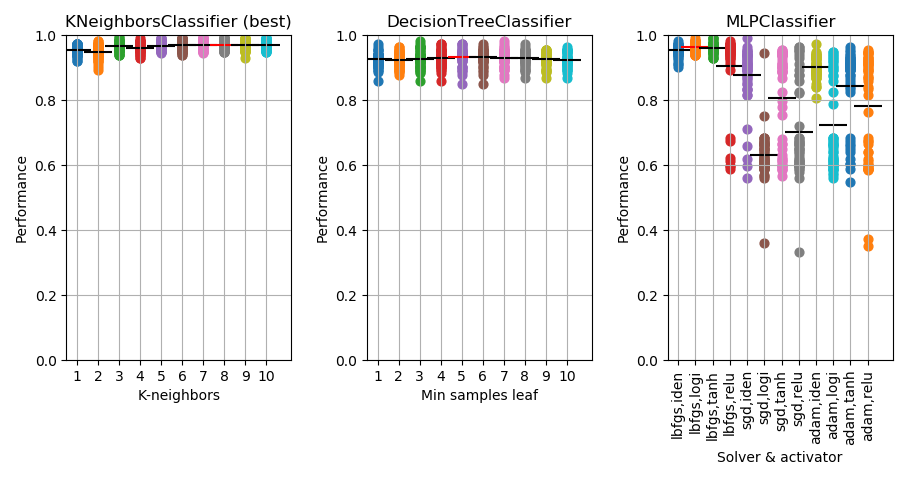
\includegraphics[width=1\textwidth]{ex2_breastcancer}
    \end{center}
    \caption{Résultat de la validation croisée sur les données du cancer du sein}
    \label{Résultat de la validation croisée sur les données du cancer du sein}
\end{figure}

De manière générale, les 3 méthodes, avec les paramètres adéquats, donnent des résultats satisfaisants.
En effet, la plupart des variations donne un score moyen qui dépasse les 90\%. \\

La méthode des k-plus proches voisins est ici pour peu la meilleure méthode.
La variation du paramètre \textit{K} n'affecte que de quelques pourcents le score moyen.
Par ailleurs, on peut observer qu'après $K = 6$,
le score moyen est stable et la variation du paramètre n'a plus aucun effet. \\

Concernant la méthode des arbres de décision,
on remarque que la courbe construite à partir des scores moyens produit un pic lorsque
le nombre d'élément minimum dans un nœud feuille est de 5.
On peut donc en déduire que les données peuvent facilement être regroupé par 5.
Ceci explique également le \textit{K} obtenu pour la méthode des k-plus proches voisins. \\

Quant au Perceptron multi-couche, les différents solvers donnent des résultats bien différents,
alors que changer la fonction d'activation ne produit que peu d'effet,
excepté certaines combinaisons,
comme le solver \textit{sdg (stochastic gradient descent)} et la fonction d'activation \textit{logistic (fonction sigmoid)} qui
produit un effet désastreux.
Cependant, cette même fonction d'activation marche très bien avec le solver \textit{lbfgs},
produisant un résultat similaire à la méthode des k-plus proches voisins.

\newpage

% -----------------------------------------------------------------------------
\subsection{Données des vins}

Voici ci-dessous le résultat de la validation croisée pour les méthodes citées sur les données des vins:

\begin{figure}[H]
    \begin{center}
        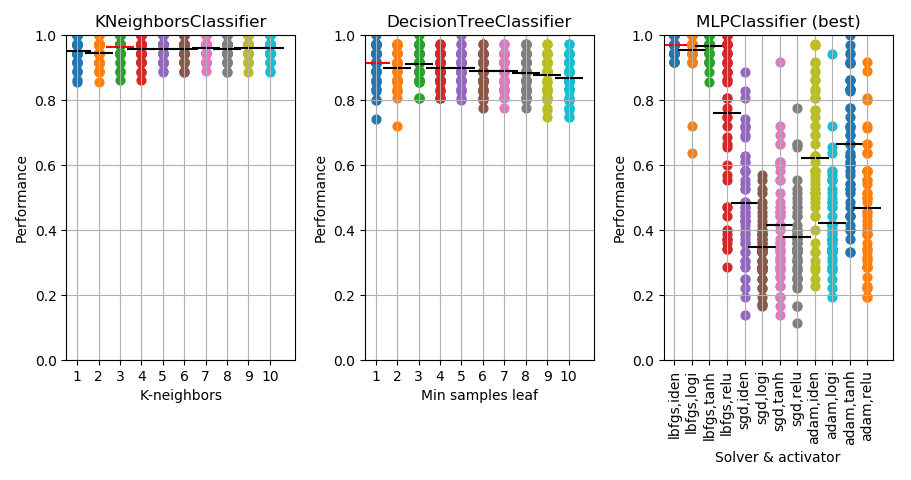
\includegraphics[width=1\textwidth]{ex2_wine}
    \end{center}
    \caption{Résultat de la validation croisée sur les données des vins}
    \label{Résultat de la validation croisée sur les données des vins}
\end{figure}

Par rapport au données du cancer du sein,
on remarque immédiatement que les scores sont de manière générale plus étalés.
On peut donc en déduire que ces données se regroupent moins facilement.
On peut par ailleurs bien l'observer avec la méthode des arbres de décision,
où l'on voit que la meilleure variations est lorsqu'il n'y a qu'un seul élément dans un nœud feuille. \\

Pour ces données, la meilleure méthode est le Perceptron multi-couche.
Nous retrouvons encore le solver \textit{lbfgs},
mais cette fois avec la fonction d'activation \textit{identité} au lieu de la \textit{sigmoid}.
On voit également que les autres solvers, quelque soit la fonction d'activation, sont mauvais avec ces données. \\

Pour peu, la méthode des k-plus proches voisins n'est pas la meilleure.
Ceci dit, toutes les variations de cette méthode sont bonne.
Le paramètre \textit{K} n'a que peu d'effet.

\newpage

% -----------------------------------------------------------------------------
\section{Classification supervisée libres}

La partie 3 de ce travail suit le même principe que la partie 2 (voir section \ref{part2}),
mais les 3 méthodes ainsi que les données sont à choix. \\

Les données choisies sont celles sur les feuilles de plantes\footnote{\url{https://archive.ics.uci.edu/ml/datasets/Leaf}}. \\

Les 3 méthodes sont les suivantes:
\begin{itemize}
    \item support vector machines;
    \item forêts aléatoires;
    \item arbres de décision. \\
\end{itemize}

Pour la méthode des support vector machines, tous les noyaux sont testés. \\
Pour la méthode des forêts aléatoires ainsi que celle des arbres de décision,
le nombre minimum d'échantillon dans une feuille est fait varié de 1 à 10 compris. \\

\begin{figure}[H]
    \begin{center}
        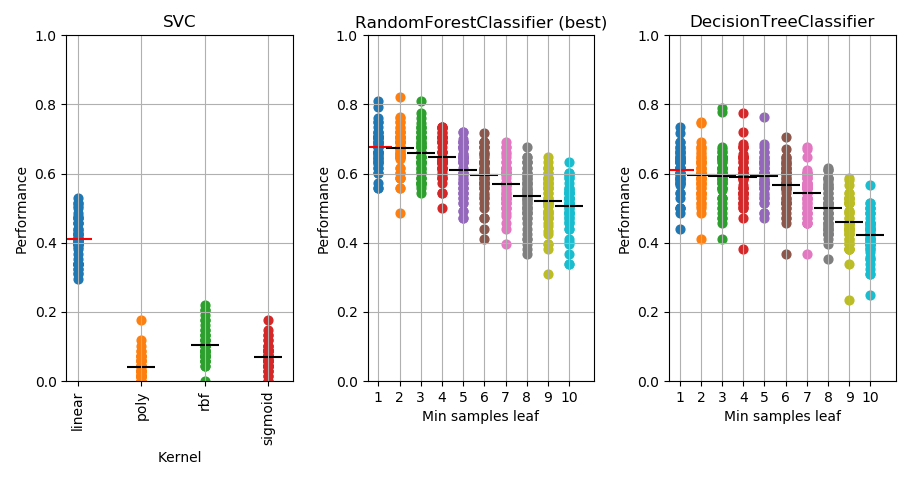
\includegraphics[width=1\textwidth]{ex3}
    \end{center}
    \caption{Résultat de la validation croisée sur les données des feuilles de plantes}
    \label{Résultat de la validation croisée sur les données des feuilles de plantes}
\end{figure}

\newpage

% -----------------------------------------------------------------------------
\section{Conclusion}

\end{document}
